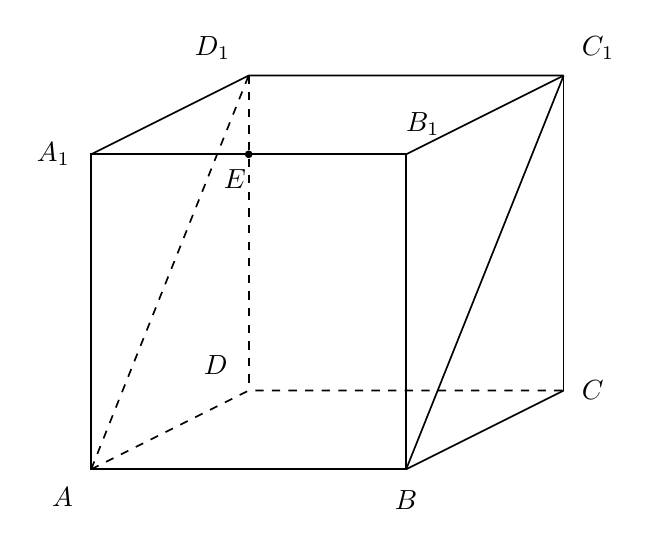
\begin{tikzpicture}[x=1cm,y=1cm,line width=.6pt,font=\normalsize]
\coordinate (A1) at (0,4);
\coordinate (B1) at (4,4);
\coordinate (C1) at (6,5);
\coordinate (D1) at (2.0000000000,5.0000000000);
\coordinate (A) at (0,0);
\coordinate (B) at (4,0);
\coordinate (C) at (6,1);
\coordinate (D) at (2,1);
\coordinate (E) at (2.0000000000,4.0000000000);
% front face
\draw (A1) -- (B1) -- (B) -- (A) -- cycle;
% top face
\draw (A1) -- (D1) -- (C1);
\draw (B1) -- (C1);
% right face
\draw (C1) -- (C);
\draw (B) -- (C);
% plane diagonal B-C1
\draw (B) -- (C1);
% hidden dashed
\draw[dashed] (D1) -- (D);
\draw[dashed] (A) -- (D) -- (C);
\draw[dashed] (A) -- (D1);
\fill (E) circle (1.4pt);
\node[left,xshift=-4pt] at (A1) {$A_{1}$};
\node[above,xshift=6pt,yshift=3pt] at (B1) {$B_{1}$};
\node[above right,xshift=3pt,yshift=2pt] at (C1) {$C_{1}$};
\node[above left,xshift=-3pt,yshift=2pt] at (D1) {$D_{1}$};
\node[below left,xshift=-3pt,yshift=-3pt] at (A) {$A$};
\node[below,xshift=0pt,yshift=-4pt] at (B) {$B$};
\node[right,xshift=3pt] at (C) {$C$};
\node[above left,xshift=-4pt,yshift=2pt] at (D) {$D$};
\node[below=3pt,xshift=-5pt,yshift=1pt] at (E) {$E$};
\end{tikzpicture}
